\section{Active \TTTS{} for Hyper-Parameter Optimization}\label{sec:dttts.algorithm}

In this section, we introduce a new algorithm for \gls{bai} in an infinite bandit model, that is an adaptation of \gls{ttts}{} (see Chapter~\ref{CHAP:T3C}). Unlike \SHA{} that requires the knowledge of the total budget to operate, \gls{ttts}{} is particularly appealing as it does not need to have it. Remember that such algorithms are referred to as \emph{anytime}. Besides, it is known to be optimal in a Bayesian (asymptotic) sense (see Chapter~\ref{CHAP:T3C}).

Recall that as a Bayesian algorithm, \gls{ttts} uses a prior distribution $\Pi_0$ over the vector of means of the $K$ arms, $\bmu \triangleq (\mu_1,\cdots,\mu_K)$, which can be updated to a posterior distribution $\Pi_n$ after $n$ observations. 

We consider Bernoulli bandit model in the rest of this chapter. Under Bernoulli bandit model, arm $i$ produces a reward $r_{n,i}=1$ with probability $\mu_i$, and $r_{n,i}=0$ with probability $1-\mu_i$ when sampled at round $n$. Given independent uniform prior for the mean of each arm, the posterior distribution on $\bmu$ is a product of $K$ Beta distributions: $\Pi_n = \bigotimes_{i=1}^{K} \texttt{Beta}(1+S_{n,i},N_{n,i}-S_{n,i}+1)$, where $N_{n,i}$ is the number of selections of arm $i$ until round $n$ and $S_{n,i}$ is the sum of rewards obtained from that arm. 
%At each round $n$, \gls{ttts} chooses one arm from the following two candidates to evaluate: (1) it first samples a parameter ${\bm\theta}$ from $\Pi_{t-1}$, and the first candidate is defined as $I_n^{\,(1)} \eqdef \argmax_{i\in\cX} {\theta}_i$, (2) it repeatedly samples new ${\bm\theta}'$ until $I_n^{\,(2)} \eqdef \argmax_{i\in\cX} \theta_i'$ is different from $I_n^{\,(1)}$. \gls{ttts} depends on a parameter $\beta \in (0,1)$. In particular, the algorithm selects $I_n = I_n^{\,(1)}$ with probability $\beta$ and $I_n = I_n^{\,(2)}$ with probability $1-\beta$.

\paragraph{Best of best-arm identification.}

We further motivate experimentally why we choose to build new algorithms upon \gls{ttts} in this section. 

We consider here some fixed-budget and anytime \gls{bai} algorithms, including uniform allocation~\citep{bubeck2009pure}, \UCBE{} and \SR{}~\citep{audibert2010budget}, \UGapE~\citep{gabillon2012ugape}, \SHA{}, \TS{} with a MPA strategy of decision (see Section~\ref{sec:mab.bai.decision}), \gls{ttts}{}, \ATLUCB{}~\citep{jun2016atlucb}.

We use 8 problem instances proposed by~\cite{audibert2010budget}, all settings consider Bernoulli bandits, and we compare their trending \emph{simple regret} averaged on 1000 trials. The results are shown in Fig.~\ref{fig:bai}.

\begin{itemize}
	\item Setting 1: $\mathbf{\mu_1}=0.5, \mathbf{\mu_{2:20}}=0.4, \operatorname{budget}=2000$
	\item Setting 2: $\mathbf{\mu_1}=0.5, \mathbf{\mu_{2:6}}=0.42, \mathbf{\mu_{7:20}}=0.38, \operatorname{budget}=2000$
	\item Setting 3: $\mathbf{\mu}=[0.5, 0.3631, 0.449347, 0.48125839], \operatorname{budget}=2000$
	\item Setting 4: $\mathbf{\mu}=[0.5, 0.42, 0.4, 0.4, 0.35, 0.35], \operatorname{budget}=600$
	\item Setting 5: $\mathbf{\mu_1}=0.5, \mathbf{\mu_i}=\mathbf{\mu_1}-0.025i, \forall i\in\{2\ldots15\}, \operatorname{budget}=4000$
	\item Setting 6: $\mathbf{\mu_1}=0.5, \mathbf{\mu_2}=0.48, \mathbf{\mu_{3:20}}=0.37, \operatorname{budget}=6000$
	\item Setting 7: $\mathbf{\mu_1}=0.5, \mathbf{\mu_{2:6}}=0.45, \mathbf{\mu_{7:20}}=0.43, \mathbf{\mu_{7:20}}=0.38, \operatorname{budget}=6000$
	\item Setting 8: $\mathbf{\mu_1}=0.5, \mathbf{\mu_{2:6}}=0.45, \mathbf{\mu_{7:20}}=0.43, \mathbf{\mu_{7:20}}=0.38, \operatorname{budget}=12000$
\end{itemize}

\begin{figure}[ht]
  \centering
  \begin{subfigure}[t]{0.25\textwidth}
    \centering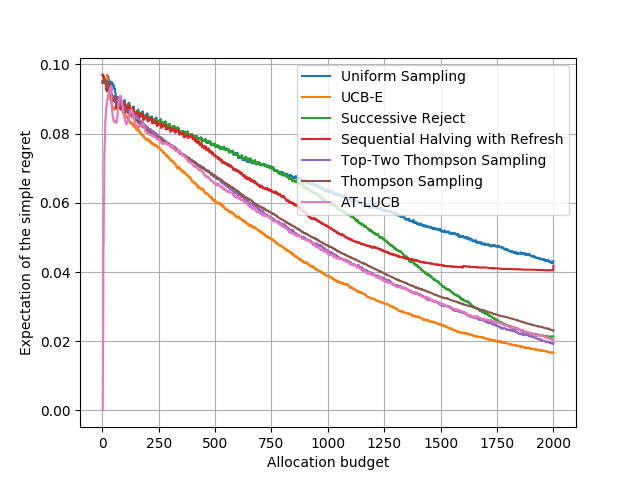
\includegraphics[width=\textwidth]{Chapter6/img/bai/setting1.png}
    \caption{Problem 1}
  \end{subfigure}%
  \begin{subfigure}[t]{0.25\textwidth}
    \centering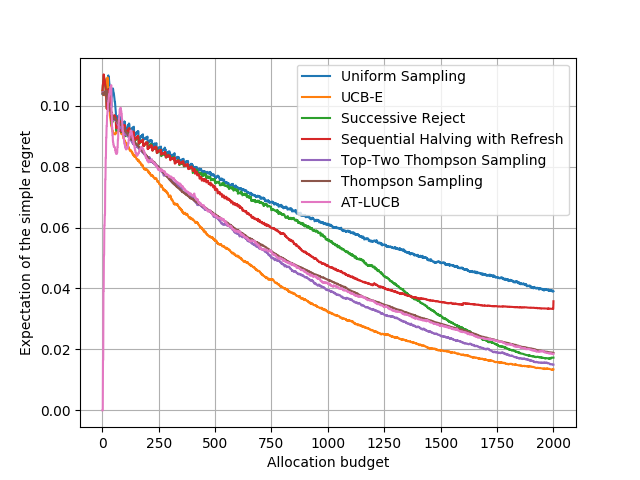
\includegraphics[width=\textwidth]{Chapter6/img/bai/setting2.png}
    \caption{Problem 2}
  \end{subfigure}
  \begin{subfigure}[t]{0.25\textwidth}
    \centering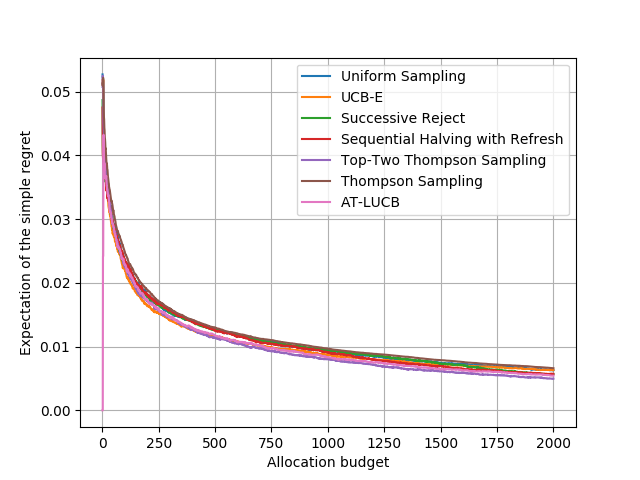
\includegraphics[width=\textwidth]{Chapter6/img/bai/setting3.png}
    \caption{Problem 3}
  \end{subfigure}%
  \begin{subfigure}[t]{0.25\textwidth}
    \centering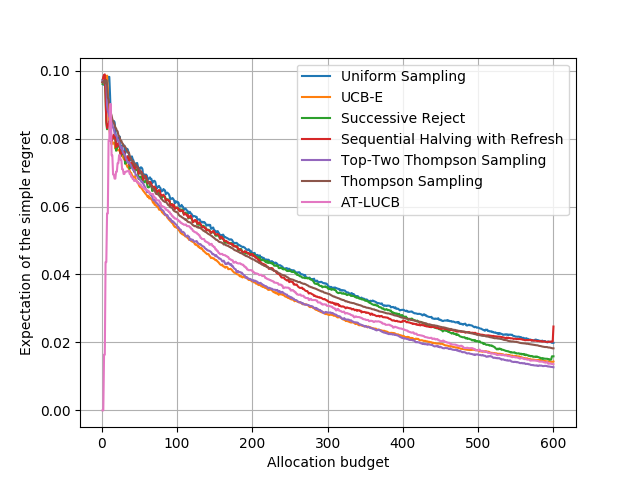
\includegraphics[width=\textwidth]{Chapter6/img/bai/setting4.png}
    \caption{Problem 4}
  \end{subfigure}
  \begin{subfigure}[t]{0.25\textwidth}
    \centering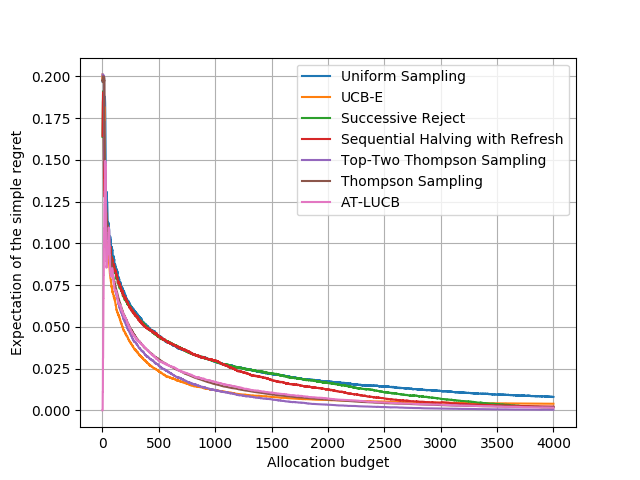
\includegraphics[width=\textwidth]{Chapter6/img/bai/setting5.png}
    \caption{Problem 5}
  \end{subfigure}
  \begin{subfigure}[t]{0.25\textwidth}
    \centering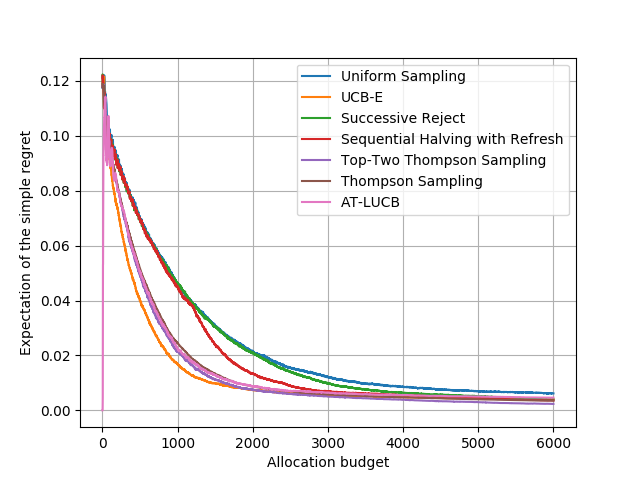
\includegraphics[width=\textwidth]{Chapter6/img/bai/setting6.png}
    \caption{Problem 6}
  \end{subfigure}
  \begin{subfigure}[t]{0.25\textwidth}
    \centering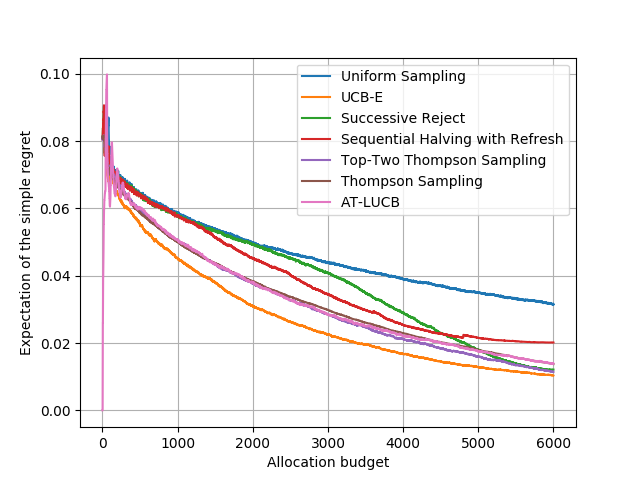
\includegraphics[width=\textwidth]{Chapter6/img/bai/setting7.png}
    \caption{Problem 7}
  \end{subfigure}
  \begin{subfigure}[t]{0.25\textwidth}
    \centering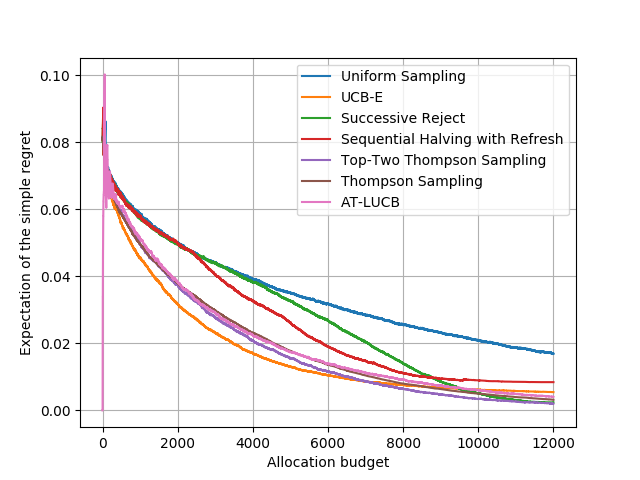
\includegraphics[width=\textwidth]{Chapter6/img/bai/setting8.png}
    \caption{Problem 8}
  \end{subfigure}
  \caption{Comparing different fixed-budget and anytime BAI algorithms.}
  \label{fig:bai}
\end{figure}

In these experiments, \gls{ttts} are always beating or at least performing as well as its competitors. It thus seems to be a good candidate to be further investigated.

Note that \gls{ttts} can also be used for bandit settings in which the rewards are bounded in $[0,1]$ by using a binarization trick first proposed by~\cite{agrawal2012analysis}: When a reward $r_{n,i} \in [0,1]$ is observed, the algorithm is updated with a fake reward  
\[
    r'_{n,i} \sim \texttt{Bern}(r_{n,i}) \in \{0,1\}\,.
\]
\gls{ttts} can thus be used for \gls{bai} for a \emph{finite} number of arms that with rewards in $[0,1]$. We now present a simple way of extending \gls{ttts}{} to deal with an infinite number of arms, namely \gls{dttts}.

\paragraph{Dynamic \TTTS{}.}

%The rationale behind \DTTTS is the following. 

In an infinite bandit algorithm, at each round, we either query a new arm from the reservoir \emph{and sample it}, or re-sample a previous arm. In a Bayesian setting, we can also imagine that at each round, an arm is queried from the reservoir and added with a \textit{uniform prior} to the list of queried arms, \emph{regardless of whether it is sampled or not}. Then, at round $t$, \DTTTS consists in running \gls{ttts} on these $t$ arms, out of which several are endowed with a uniform prior and have never been sampled. 

Leveraging the fact the the maximum of $k$ uniform distribution has a \texttt{Beta}($k,1$) distribution and that \gls{ttts} only depends on the maxima of posterior samples, we give the following equivalent implementation for \DTTTS (Algorithm~\ref{alg:dttts}). Letting $\cL_n$ be the list of arms that have been queried  from the reservoir and sampled \textit{at least once} before round $t$, at round $t$ we run \gls{ttts} on the set $\cX_n \triangleq \cL_n \cup \{\mu_0\}$ where $\mu_0$ is a pseudo-arm with posterior distribution \texttt{Beta}($n-k_n, 1$), where $k_n\triangleq|\cL_n|$.  

\begin{algorithm}[ht]
\centering
\caption{Sampling rule of Dynamic \DTTTS{}}
\label{alg:dttts}
\begin{algorithmic}[1] %[1] enables line numbers
    \State {\bfseries Input: } $\beta$; $B$ (total budget); $\nu_0$
    \State {\bfseries Initialization: } $\mu_1 \sim \nu_0$; $t \gets 0$; $\cX \gets \{\mu_0,\mu_1\}$; $m\gets1$; $S_0, N_0 \gets 0$; $S_1 \sim \texttt{Bern}(\mu_1)$, $N_1 \gets 1$\
    
    \While{$n < B$}
	    \State $\forall i=0,\dots,m$, $\theta_i \sim \texttt{Beta}(S_i+1,N_i-S_i+1)$; $U \sim \cU([0,1])$
	    \State $I^{\,(1)} \gets \argmax_{i=0,\dots,m} \theta_i$
	    \If{$U > \beta$}
	        \While{$I^{\,(2)} = I^{\,(1)}$} 
	            \State $\forall i=0,\dots,m, \theta_i' \sim \texttt{Beta}(S_i+1,N_i-S_i+1)$
	            \State $I^{\,(2)} \leftarrow \argmax_{i=0,\dots,m}\theta_i'$ 
	        \EndWhile
	        \State $I^{\,(1)} \gets I^{\,(2)}$
	    \EndIf
	    \If{$I^{\,(1)} \neq 0$}
	        \State $Y \leftarrow$ \text{Evaluate arm} $I^{\,(1)}$; $X \sim \texttt{Bern}(Y)$ 
	        \State $S_{I^{\,(1)}} \gets S_{I^{\,(1)}} + X$; $N_{I^{\,(1)}} \gets N_{I^{\,(1)}} + 1$; $S_0 \gets S_0 + 1$
	    \Else
            \State $\mu_{m+1}\sim \nu_0$; $\cX \gets \cX \cup \{\mu_{m+1}\}$; 
            \State $Y \leftarrow$ \text{Evaluate arm} $m+1$; $X \sim \texttt{Bern}(Y)$
           	\State $S_{m+1} \gets X$; $N_{m+1}
           	\gets 1$; $m \gets m + 1$
 	   \EndIf
  	   \State $t\gets t+1$
    \EndWhile
\end{algorithmic}
\end{algorithm}

It remains to decide how to recommend the arm as our best guess. It is obviously not a good idea to output the arm with the best empirical means since some lately sampled arms may have very high empirical mean with no confidence. In this chapter, we choose the most natural recommendation strategy for Bayesian algorithms that outputs the arm with the largest optimal action probability (see Section~\ref{sec:t3c.algorithm}). Let $\Theta_i$ be the subset of the set $\Theta$ of possible mean vectors such that arm $i$ is optimal, $\Theta_i \eqdef \big\{ \btheta\in\Theta \,|\, \theta_i > \max_{j\neq i}\theta_j \big\}$, the posterior probability that arm $i$ is optimal after round $t$ is defined as $\Pi_{n}(\Theta_i)$. At any time $n$, we therefore recommend  arm 
\[
    J_n \eqdef \argmax_{i\in\cX} \Pi_{n}(\Theta_i)\,.
\]

\paragraph{Hyper-\TTTS{}.}

We present here also another simple way of extending \gls{ttts} to deal with an infinite number of arms, namely \texttt{Hyper}-\gls{ttts} or \HTTTS, a variant of \Hyperband in which \texttt{SHA} is replaced by \gls{ttts}. This algorithm, whose sampling rule is formally stated as Algorithm~\ref{alg:httts}, runs $s_{\max}$ batches of \gls{ttts} with different number of arms $n$ and each batch with a same budget $T=\ceil{B/s_{\max}}$ with $B$ the total budget. The number of arms within each bracket is decreasing with an exponential rate of~$\gamma$. One inconvenience of this algorithm is that $s_{\max}$ and~$\gamma$ still need to be tuned (in practice, we use the same tuning as the one of \Hyperband). \DTTTS is thus proposed to circumvent this issue. 

\begin{algorithm}[ht]
\centering
\caption{Sampling rule of \HTTTS{}}
\label{alg:httts}
\begin{algorithmic}[1] %[1] enables line numbers
    \State {\bfseries Input: } $\beta$; $\gamma$; $B$; $s_{\operatorname{max}}$; $\nu_0$
    \State {\bfseries Initialization: } $T=\floor{B/s_{\operatorname{max}}}$

    \For{$s \leftarrow s_{\operatorname{max}}$ to $0$}
    	\State $K = \ceil{\frac{s_{\operatorname{max}}+1}{s+1}\gamma^s}$
    	\State $\cX \leftarrow \{i=1,\ldots,K: \mu_i\sim\nu_0\}$; $t=0$
    	\While{$t < T$}
    		\State \text{Sample} $\btheta \sim \Pi_n$
            \State $I^{(1)} \leftarrow \argmax_{i\in\cX}\theta_i$
    	    \State \text{Sample} $b \sim \operatorname{Bernoulli}(\beta)$
    	    \If{$b = 1$}
    	        \State $Y \leftarrow$ \text{Evaluate arm} $I^{(1)}$
    	    \Else
    	        \While{$I^{(2)} = I^{(1)}$} 
    	            \State $\forall i\in\cX, \theta_i' \sim \texttt{Beta}(S_i+1,N_i-S_i+1)$
    	            \State $I^{(2)} \leftarrow \argmax_{i \in \cX}\theta_i'$ 
    	        \EndWhile
    	        \State $I^{(1)} \gets I^{(2)}$
    		    \State $Y \leftarrow$ \text{Evaluate arm} $I^{(1)}$
    	    \EndIf
    	    \State $X \sim \texttt{Bernoulli}(Y)$ 
    	    \State $S_{I^{(1)}} \gets S_{I^{(1)}} + X$; $N_{I^{(1)}} \gets N_{I^{(1)}} + 1$
    		\State $t = t+1$
        \EndWhile
    \EndFor
\end{algorithmic}
\end{algorithm}

